\subsection{Overview}
Arduino refers both to the microcontroller board used to interface with sensors and actuators and to the software used to program it.\\

As a microcontroller, an Arduino is a relatively cheap development board useful for controlling many input and output pins, either digital or analog, in a single board solution that plugs directly into the computer over USB.\\

As a software environment, it provides a simple IDE with many code examples, a bootloader to program microcontroller chips directly with almost no external components and a growing user community that creates libraries for different sensors and communication protocols among others.\\

All Arduino programs follow the structure presented in Figure \ref{arduinoSkeleton}, namely one Setup function and one Loop function. The first is executed only once at the beginning of the program, while the latter is equivalent to a "while(1)" block, meaning that any code entered into it will be repeated until the microcontroller shuts down or is reset.\\

\begin{figure}[H]
      \centering
      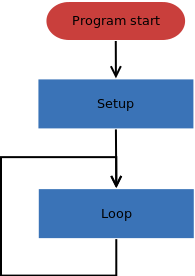
\includegraphics[scale=.8]{images/Diagrams/arduinoSkeleton.png}
      \caption{Arduino code skeleton }
      \label{arduinoSkeleton}
\end{figure}
\bigskip



%%%%%%%%%% FLOWCHART%%%%%%%%%%%%%%%%%%%%%%%%%%%%%%%%%%%%%%%%%%%%%%%%%%%%%%%
\newpage
\subsection{Code}

In this section the code written for the robot's controller will be explained. A flowchart diagram of the program is illustrated by Figure \ref{arduinoFlowchart}.\\

	\begin{itemize}
        
	    \item As it can be seen, the Arduino first defines all the robot's data, including the motor, servomotor and communication pins. This ensures the microcontroller knows where to send each datum once the user connects to the robot.\\

		\item The program then enters its Loop function. Here it will check if the serial port is available, eg the user has sent a stream of data. Once the port is available, the Read function is called, which stores every byte received into a string to be used later. Once the reading has ended the code checks if it has received a special end-of-line character that signals the end of the data stream. If all the data was retrieved the code moves on to the next function.\\

		\item The Parse function is called upon next. This function's purpose is to break and convert the previously stored string into the corresponding variables needed by each element, taking into account their sizes and types. Hence, it transforms one line of numbers into many parameters such as rotation angle, arm selection or movement direction which will be used by the next function.\\

		\item With the data correctly formatted, the program executes the Process function which is where the "thinking" is done. Here are defined all the rules the robot must follow, such as knowing which claw to close depending on the side chosen by the user but closing both if the symmetry box was checked. It takes the data provided by the previous function and processes them to end up with a structured list of variables ready to be assigned to each element.\\

		\item In the next step the Write function is called. This very simple function goes through the previous list assigning each variable to the corresponding element's assigned pins.\\

		\item Finally, the code clears the initial string to make space for new data, resets the flag informing of the correct retrieval from the serial port and proceeds to the next iteration within the Loop function, restarting the process.\\

	\end{itemize}

	\begin{figure}[H]
			\centering
			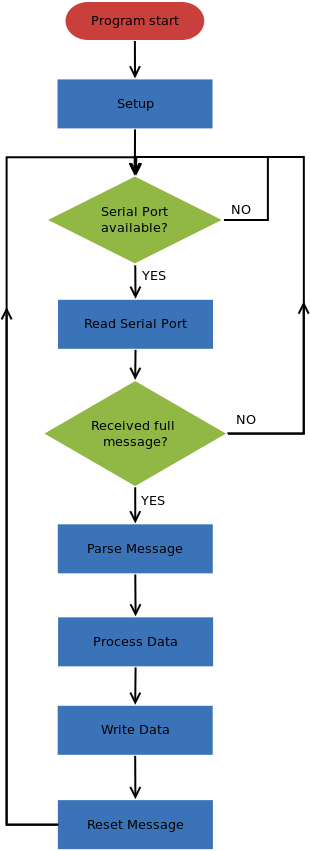
\includegraphics[scale=0.75]{images/Diagrams/arduino2.png}
			\caption{Arduino program flowchart }
			\label{arduinoFlowchart}
	\end{figure}
	\bigskip


